\chapter{组织你的文本}

从这一章开始,我们将要深入 \LaTeX 编辑的各个方面,首先来看\LaTeX 文档中文本的编辑和组织,在探究中,我们会从一个一个空格、一个标点开始分析,但深入细节的同时也不要忘记整个文档的结构和组织性,要见树木更见森林。

\section{文字与符号}

\subsection{字斟句酌}

简单正文的输入没有太多特别之处,\TeX 传统上使用扩展 ASCII 字符集,较新的\TeX 引擎使用 UTF-8 编码。在接受的字符集之内,除了个别特殊符号,大部分字符可以直接录入。

\subsubsection{从字母表到单词}

在 \LaTeX 中可以从标准键盘上直接打出 26 个字母的大小写形式。当然,从字母表到单词只有一步之遥,即用空格和标点把字母分开。但事实上总免不了要遇到一些稀奇古怪的词汇或人名,试试输入下面的词:
\begin{center}
    café \quad Gödel \quad Antonín Dvořák \quad Øster Vrå \quad Kιrkağaç
\end{center}

或者这些:
\begin{center}
    χαïδεύηζ \quad КpЮковa
\end{center}

上面的例子中,前一组词是来自拉丁字母,但明显增加了许多符号;后一组则是希腊语词汇和俄语人名。我们常用的字母表包括扩展的拉丁字母、希腊字母和西里尔字母( Cyrillic alphabet ),这比标准键盘上所能直接输入的 52 个字母要多得多。不过不用担心,数以万计的汉字我们也搞定了,区区几个字母也不在话下。

解决输入超过 ASCII 码范围的字母的问题有传统和现代两类方案,先来看一下现代的方案。

现代的方案就是使用 UTF-8 编码直接输入。在 XeTeX 这样的排版引擎下, UTF-8 编码是原生的,不需要任何多余的设置:

\begin{minipage}[t]{0.45\textwidth}
    \begin{lstlisting}
    % UTF-8 编码
    café \quad Gödel \quad Antonín Dvořák

    χαïδεύηζ \quad КpЮковa
    \end{lstlisting}
\end{minipage}
\hfill
\begin{minipage}[t]{0.45\textwidth}
    \vspace{0.1cm}
    \hspace{0.5cm}

    café \quad Gödel \quad Antonín Dvořák

    χαïδεύηζ \quad КpЮковa
\end{minipage}

不过,要想正确输入、显示并输出所有这些符号,仍然不是一件简单的事。

输入特殊的字母需要计算机键盘布局或输入法的支持,例如在法语键盘中(一般可以在操作系统中设置),标准键盘 7 8 9 0 位置上的字符分别是 \verb|è _ ç à| ,这种键盘布局对需要大量录入法语的人来说特别有用。如果不方便使用特殊键盘来设置,操作系统或编辑器往往还提供了“字符映射表”一类的程序或插件,可以用鼠标选取一些字符输入;中文输入法的软键盘也可以用来输入一小部分特殊的外文字母。

显示 ASCII 以外的字母表需要编辑器使用的字体的支持。大部分西文字体都支持扩展拉丁字母,如 è 、ç ,但不是所有字体都有希腊字母和西里尔字母,即使是一些罕用的拉丁字母(如 ř 也有可能缺失。编辑器常用的等宽字体中, Windows 和 Mac 系统都预装的 Courier New , Windows 下的 Consolas 、 Lucida Sans Typewriter 等都能显示上面所列的所有字母, Linux 下常用的 Bitstream Vera Sans Mono 、 Inconsolata 则只支持到扩展拉丁字母,因此配置编辑器时也需要仔细选择。

最后但却最重要的是, \TeX 系统输出时所使用的字体,也必须要能直接显示这些字母。 \LaTeX 默认的 Computer Modern 在一个字体中只覆盖很小的字符集, XeLaTeX 下默认的 Latin Modern 字体要好得多,一般都支持到拉丁字母(这通常就足够了),但希腊、西里尔这些字体需要更换其他字体。要完整显示其他语言的字母,就必须频繁地更换不同的字体,或在 \TeX 中使用覆盖更大字符集的字体。比如为了能正确显示前面例子中的三种字母,我们在前面已经设置了 Windows 系统预装的 Times New Roman 字体。

而传统的解决方案是使用特殊的命令,给字母加上重音的标记,使用特殊字母或者整体更换字母表。

所谓重音( accents ),是指加在字母上的标记,实际包括抑音符、锐音符、抑扬符等等多种符号。 \LaTeX 支持的重音标记及其命令见表\ref{tab:zhongyin},命令名称大多取象形的符号。将重音加之于普通的拉丁字母上,可以得到一大批扩展的拉丁字母。

\begin{table}[H]
    \centering
    \caption{\LaTeX 中的重音命令,以字母 o 为例}
    \label{tab:zhongyin}
    \begin{tabular}{ccccccccccc}
        \toprule
        \`o & \verb|\`o| 
        & \qquad &
        \'o & \verb|\'o| 
        & \qquad &
        \^o & \verb|\^o| 
        & \qquad &
        \"o & \verb|\"o| \\
        \~o & \verb|\~o| 
        & \qquad &
        \=o & \verb|\=o| 
        & \qquad &
        \.o & \verb|\.o| 
        & \qquad &
        \u{o} & \verb|\u{o}| \\
        \v{o} & \verb|\v{o}| 
        & \qquad &
        \H{o} & \verb|\H{o}| 
        & \qquad &
        \t{oo} & \verb|\t{oo}| 
        & \qquad &
        \r{o} & \verb|\r{o}| \\
        \c{o} & \verb|\c{o}| 
        & \qquad &
        \d{o} & \verb|\d{o}| 
        & \qquad &
        \b{o} & \verb|\b{o}| 
        & \qquad &
         &  \\
    \bottomrule
    \end{tabular}
\end{table}

使用命令可以输入的 \LaTeX 字母,见表\ref{tab:special}。其中,\i , \j 就是字母 i , j ,只是在加上重音命令时需要去掉上面的点。 \ij,\IJ,\SS 是字母连写,在默认的字体中没有区别。

\begin{table}[H]
    \centering
    \caption{\LaTeX 中的特殊字母}
    \label{tab:special}
    \begin{tabular}{ccccccccccc}
        \toprule
        \AA & \verb|\AA| 
        & \qquad &
        \aa & \verb|\aa| 
        & \qquad &
        \AE & \verb|\AE| 
        & \qquad &
        \ae & \verb|\ae| \\
        \OE & \verb|\OE| 
        & \qquad &
        \oe & \verb|\oe| 
        & \qquad &
        \SS & \verb|\SS| 
        & \qquad &
        \ss & \verb|\ss| \\
        \IJ & \verb|\IJ| 
        & \qquad &
        \ij & \verb|\ij| 
        & \qquad &
        \L & \verb|\L| 
        & \qquad &
        \l & \verb|\l| \\
        \O & \verb|\O| 
        & \qquad &
        \o & \verb|\o| 
        & \qquad &
        \i & \verb|\i| 
        & \qquad &
        \j & \verb|\j| \\
    \bottomrule
    \end{tabular}
\end{table}

如果还要输入希腊字母和西里尔字母,默认的字体就不够用了,需要更换其他编码和字体。为此,\LaTeX 提供了 babel 宏包,可以方便地同时访问多种语言的字母表。 babel 宏包可带有一个或多个语言的可选参数,支持不同的语言,如
\begin{lstlisting}
    \usepackage[greek,english]{babel}
\end{lstlisting}
将使用英语和希腊语,其中作为最后一个参数的英语是默认语言,此时希腊语就可以用 ASCII 字符代替:
\begin{lstlisting}
    \textgreek{abcde}
\end{lstlisting}
上述代码输出 αβζδε 。需要少量俄文的西里尔字母,可以换用 OT2 编码的字体德奥。

例如:

\begin{minipage}[t]{0.45\textwidth}
    \begin{lstlisting}
% 导言区 \usepackage[OT2,OT1]{fontenc}
{\fontencoding{OT2} \selectfont ABCabc}
    \end{lstlisting}
\end{minipage}
\hfill
\begin{minipage}[t]{0.45\textwidth}
    \vspace{0.1cm}
    \hspace{0.5cm}
    {\fontencoding{OT2} \selectfont ABCabc}
\end{minipage}
如果排版全文是俄文的文章,也可以用 \verb|russian| 参数使用 \verb|babel| 宏包,不过输入时就不使用 ASCII 码,而使用俄文专用的编码。由于这些语言很少用,这里不做更多说明。

使用 pdfTeX 这样的传统排版引擎也可以使用 UTF-8 编码输入文字,此时需要使用 inputenc 宏包并选用 \verb|utf8| 选项,它会将 UTF-8 的输入编码自动转换为当前字体编码所对应的符号,字体编码的设置仍然与原来一样,如:
\begin{lstlisting}
    % coding: utf-8
    % pdflatex 命令编译
    \documentclass{article}
    \usepackage[OT2,OT1]{fontenc}
    \usepackage[utf8]{inputenc}
    \begin{document}
    café \quad Gödel
    {\fontencoding{OT2} \selectfont КpЮковa}
    \end{document}
\end{lstlisting}

\LaTeX 在排版中会将单词中的一些字母连写成为一个符号,即连字 ( ligature )。连字的有无和多少一般是由使用的字体决定的,在默认的 Computer Modern 和 Latin Modern 字体中,小写字母组合 \verb|ff,fi,fl,ffi,ffl| 都有连字:

\begin{minipage}[t]{0.45\textwidth}
    \begin{lstlisting}
    differ find flight difficult ruffle 
    \end{lstlisting}
\end{minipage}
\hfill
\begin{minipage}[c]{0.45\textwidth}
    \hspace{0.5cm}
    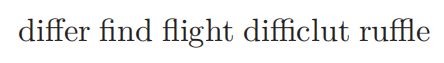
\includegraphics[width=0.6\textwidth]{连字1.png}
\end{minipage}

本书中主要使用的 Times 字体则只有 \verb|fi| 和 \verb|fl| 的连字 ( fi,fl),而一些专业字体可能用的更多:

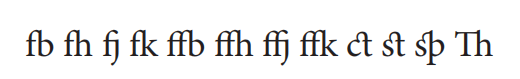
\includegraphics[width=0.3\textwidth]{连字2.png}

偶尔出于意义或美观的考虑,需要取消连字。此时可以借用\verb|\/|命令。

\begin{minipage}[t]{0.45\textwidth}
    \begin{lstlisting}
    fleet f\/leet
    \end{lstlisting}
\end{minipage}
\hfill
\begin{minipage}[b]{0.45\textwidth}
    \hspace{0.5cm}

    fleet f\/leet
\end{minipage}

使用 XeLaTeX 引擎, OpenType 字体时,可以方便地使用 fontspec 宏包的 \verb|Ligature| 字体选项选择连字的有无和程度。

\subsubsection{正确使用标点}

在键盘上,可以直接使用的符号有 16 种:

, \quad . \quad ; \quad : \quad ! \quad ? \quad ` \quad ' \quad ( \quad ) \quad [ \quad ] \quad - \quad /  \quad * \quad @

标点\ ,\ .\ ;\ :\ !\ ?\ 用来分隔句子或部分句子,在每个标点之后应该加上空格,以保证正确的距离和换行。在特殊情况下,这些标点有空格还有一些更微妙的关系。

引号在 \LaTeX 中用 \verb|`|和 \verb|'| 两个符号表示。单引号就用一遍,双引号用两遍。如果遇到单引号和双引号连续出现的情形,则在中间用 \verb|\,|命令分开:

\begin{minipage}[t]{0.45\textwidth}
    \begin{lstlisting}
    ``\,`A' or `B?' \,'' he asked.
    \end{lstlisting}
\end{minipage}
\hfill
\begin{minipage}[t]{0.45\textwidth}
    \vspace{0.1cm}
    \hspace{0.5cm}
    ``\,`A' or `B?' \,'' he asked.
\end{minipage}
这里\verb|\,| 命令产生很小的间距,注意\LaTeX 并不会忽略以符号命名的宏前后的空格,所以在它前后都不要加多余的空格。符号\verb|'| 同时也是表示所有格和省字的撇号 ( apostrophe ,如 ``It's Knuth's book'' )。

引号和括号通常要在前后加空格分割单词。逗号、句号等标点何时放在引号和括号内,何时放在引号和括号外,可参见英文写作的格式指导。

除了在数学模式中表示减号,符号 - 在\LaTeX 正文中也有多种用途:单独使用时它是连字符( hyphen );两个连用( -- ),是 en dash ,用来表示数字范围;三个连用 ( --- ),是 em dash ,即破折号:

\begin{minipage}[t]{0.45\textwidth}
    \begin{lstlisting}
        
    An inter-word dash or , hyphen, as in X-ray.

    A medium dash for number ranges, like 1--2.

    A punctuation dash --- like this.
    \end{lstlisting}
\end{minipage}
\hfill
\begin{minipage}[t]{0.45\textwidth}
    \vspace{0.1cm}
    \hspace{0.5cm}

    An inter-word dash or , hyphen, as in X-ray.

    A medium dash for number ranges, like 1--2.

    A punctuation dash --- like this.
\end{minipage}

不过,按中文写作习惯,表示数字范围也常使用符号 $\sim$ (\verb|$\sim$|) ,有时也用汉字的全角破折号或半个汉字破折号。

西文的省略号( ellipsis )使用\verb|\ldots| 或 \verb|\dots| 命令产生,相比直接输入三个句号,它所拉开的距离要合理些:

\begin{minipage}[t]{0.45\textwidth}
    \begin{lstlisting}
    Good: One, two, three \ldots

    Bad: One, two, three...
    \end{lstlisting}
\end{minipage}
\hfill
\begin{minipage}[t]{0.45\textwidth}
    \vspace{0.1cm}
    \hspace{0.5cm}

    Good: One, two, three \ldots

    Bad: One, two, three...
\end{minipage}

\verb|\ldots| 和 \verb|\dots| 命令在正文中是等价的,它们会在每个点后面增加一个小的间距,因而直接在 \verb|\ldots| 后面再加逗号、句号、叹号等标号,也能得到正确的间距。西文省略号的用法在不同的格式手册中往往有详细规定,通常在句中使用时,前后都要加空格,而在句末使用则应该使用 4 个点。这是因为 \verb|\ldots| 的后面也有间距,所以使用\verb|H\ldots.| 能得到正确的 “ H\ldots. ”,但直接使用 \verb|H \ldots\ H| 却将得到错误的间距 “ H \ldots\ H ”(后一个间距比前面大 )。解决的办法是把省略号放进数学模式:

\begin{minipage}[t]{0.45\textwidth}
    \begin{lstlisting}
    She $\ldots$ she got it.

    I've no idea\ldots.
    \end{lstlisting}
\end{minipage}
\hfill
\begin{minipage}[t]{0.45\textwidth}
    \vspace{0.1cm}
    \hspace{0.5cm}

    She $\ldots$ she got it.

    I've no idea\ldots.
\end{minipage}

标准键盘上不能直接录入的标点符号有10个,它们占据了主键盘上面一大排的一大半:

\~{} \quad \# \quad \$ \quad \% \quad \^{} \quad \& \quad \{ \quad \} \quad \_ \quad \textbackslash 

他们都有特殊作用,其中的许多我们已经熟知:数学模式符号 \$ 、注释符号 \% 、上标 \^{} 、分组 \{\} 、宏命令 \textbackslash,只有个别例外:

\begin{minipage}[t]{0.45\textwidth}
    \begin{lstlisting}[language = java]
    \~{} \quad \# \quad \$ \quad \% 
    \quad \^{} \quad \& \quad \{ \quad \} 
    \quad \_ \quad \textbackslash 
    \end{lstlisting}
\end{minipage}
\hfill
\begin{minipage}[t]{0.45\textwidth}
    \vspace{0.1cm}
    \hspace{0.5cm}

    \~{} \quad \# \quad \$ \quad \% \quad \^{} \quad \& \quad \{ \quad \} \quad \_ \quad \textbackslash 
\end{minipage}

可以用没有字母的重音\verb|\~{}| 和 \verb|\^{}| 输出 \~{} 和 \^{} ,但这两个符号一般不直接在普通正文中出现,而出现其他地方:可以是重音符号;可以出现在程序代码中;此外还有一个数学符号 $\sim$。

符号

| \quad < \quad > \quad + \quad =

虽然可以接受,但它们一般用在数学公式中,其文本形式的效果不好或有错,一般不直接使用它们。键盘上的双引号 \verb|"| 一般也极少使用在正文中,而常被另外定义移作他用。

中文使用的标点与西文标点不同 中文写作使用全角标点:

\begin{table}[H]
    \centering
    \begin{tabular}{ccccccccccc}
        句号 & 。或\ . & &
        逗号 & , & &
        顿号 & 、& &
        分号 & ; \\
        冒号 & : &&
        问号 & ? &&
        感叹号 & ! &&
        间隔号 & · \\ 
        单引号 & ‘ \quad ’ &&
        双引号 & “ \quad ” &&
        单书名号 & <\quad  > &&
        双书名号 & 《\quad 》 \\
        括号 & () [] ﹝﹞ &&
        省略号 & …… && 
        破折号 & —— 
    \end{tabular}
\end{table}

在计算机中使用中文输入法录入全角标点通常是很直接的。特别需要说明的是破折号( —— )和 省略号 (……),它们都占两个中文字符,在大部分输入法中可以使用 \verb|Shift+-| 和 \verb|Shift+6| 得到。

在科技文章中,为与数字、字母区分,中文的句号一般也用一个圆点表示,此时应该使用全角的“.” 而非混用西文句点。这个标点在大部分中文输入法下可能不易输入,可以先统一使用句号“。”,最后统一替换。

也有一种科技文章的写作风格,是中文与西文统一使用西文的标点,只有顿号、破折号和省略号仍用中文标点。但这样可能造成标点大小、位置与汉字对不准,以及字体风格的不统一,应该小心使用。

\LaTeX 并不会自动处理好汉字标点的宽度和间距,甚至不能保证标点的禁则(如句号不允许出现在一行的开始)。使用 XeTeX 作为排版引擎时,中文标点一般是由 xeCJK 宏包控制的。 xeCJK 提供了多种标点格式,默认是全角式,即所有标点占一个汉字宽度,只有在行末或个别标点之间进行标点挤压。还支持其他一些标点格式,可以使用\verb|\punctstyle| 命令修改:

\begin{center}
    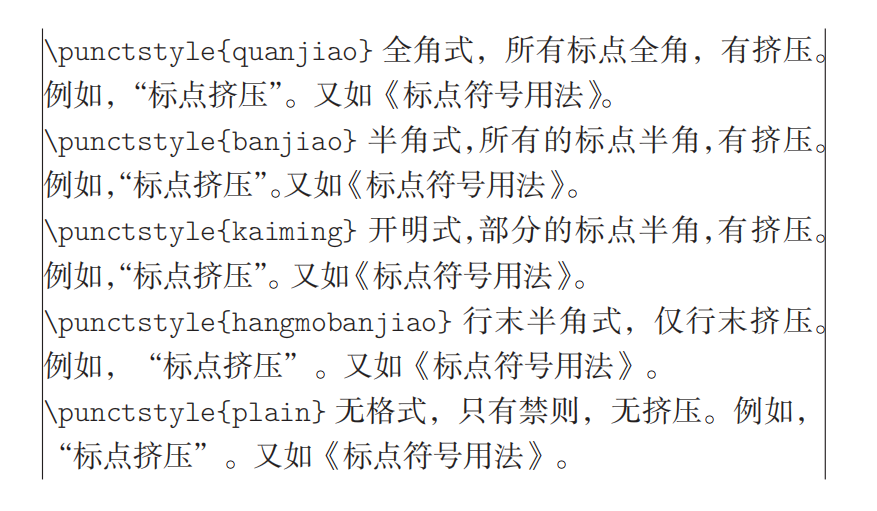
\includegraphics[width=0.6\textwidth]{标点形式.png} \centering
\end{center}

\subsubsection{看不见的字符——空格与换行}

文本中的空格起分隔单词的作用,任意多个空格的功能与一个空格相同;只有字符后面的空格是有效的,每行最前面的空格则被忽略,这样有利于复杂代码的对齐;单个换行也被看成一个空格。例如(我们仍然用 \lstinline[showspaces=true]{ } 表示空格:

\begin{minipage}[t]{0.45\textwidth}
    \begin{lstlisting}[showspaces=true]
This is     a short
sentence.  This is
             another.
\end{lstlisting}
\end{minipage}
\hfill
\begin{minipage}[c]{0.45\textwidth}
This is     a short
sentence.  This is
             another.
\end{minipage}

以字母命名的宏,后面空格会被忽略。如果需要再命令后面使用空格,可以使用\lstinline[showspaces=true]{\ },它表示两个普通字母间的空格距离;也可以在命令后加一个空白的分组\verb|{}|,有时也可以把命令用一个分组包裹起来:

\begin{minipage}[t]{0.45\textwidth}
\begin{lstlisting}[showspaces=true]
Happy \TeX ing. Happy \TeX\ ing.
Happy  \TeX{} ing. Happy {\TeX} ing.
\end{lstlisting}
\end{minipage}
\hfill
\begin{minipage}[t]{0.45\textwidth}
Happy \TeX ing. Happy \TeX\ ing.

Happy  \TeX{} ing. Happy {\TeX} ing.
\end{minipage}

有一种不可打断的空格,在\TeX 中称为带子( ties ),用\verb|~| 表示。 \TeX 禁止在这种空格之间分行,因而可以用来表示一些不宜分开的情况,例如:
\begin{lstlisting}
    Question~1              % 名称与编号间
    Donald~E. Knuth         % 教名之间,但姓可以断行
    Mr.~Knuth               % 称谓缩写与名字间
    function~$f(x)$         % 名字后面的短公式
    1,~2,and~3              % 序列的部分符号间
\end{lstlisting}

西文的逗号、句号、分号等标点后面应该加空格,这不仅能保证正确的间距,也能保证正确的换行。这是因为标点后如果没有空格,就不能换行。\LaTeX 在西文句末(包括句号\verb|.|问号\verb|?|和叹号\verb|!|)后面使用的距离会比单词间的距离大些,这在上面的例子中已经可以看到。更确切地说,\LaTeX 会把大写字母后的点看作是缩写标记,把小写后面的点看作是句子结束,并对它们使用不同的间距;但偶尔也有大写字母结束的句子,或小写字母的缩写,这就必须明确地告诉 \LaTeX 使用普通单词间的空格 \lstinline[showspaces=true]{\ } ,或用\verb|\@|,指明\verb|.| 是大写字母后的句末。例如:

\begin{minipage}[t]{0.45\textwidth}
\begin{lstlisting}[showspaces=true]
A sentence. And another.

U.S.A. means United States Army?

Tinker et al.\ made the double play.

Roman number XII\@. Yes.
\end{lstlisting}
\end{minipage}
\hfill
\begin{minipage}[t]{0.45\textwidth}
A sentence. And another.

U.S.A. means United States Army?

Tinker et al.\ made the double play.

Roman number XII\@. Yes.
\end{minipage}
有时也需要整体禁止这种在标点后的不同的间距,法语排版的习惯就是如此。此时可以使用\verb|\frenchspacing| 命令来禁止标点后的额外间距。

汉字后的空格会被忽略。使用 xelatex 编译中文文档时,汉字和其他内容之间如果没有空格, xeCJK 宏包会自动添加:

\begin{minipage}[t]{0.45\textwidth}
\begin{lstlisting}[showspaces=true]
中文和English的混排效果并不依赖 space 的有无 
\end{lstlisting}
\end{minipage}
\hfill
\begin{minipage}[t]{0.45\textwidth}
    中文和English的混排效果并不依赖 space 的有无
\end{minipage}

个别时候需要忽略汉字与其它内容之间由 xeCJK 自动产生的空格,这时可以把汉字放进一个盒子里面:

\begin{minipage}[t]{0.45\textwidth}
\begin{lstlisting}[showspaces=true]
\mbox{条目}a 不同于条目b
\end{lstlisting}
\end{minipage}
\hfill
\begin{minipage}[t]{0.45\textwidth}
\mbox{条目}a 不同于条目b
\end{minipage}

还有时需要完全禁用汉字与其他内容之间的空格,这时可以使用\verb|\CJKsetecglue| 手工设置汉字与其他内容之间的内容为空\footnote{好像现在这个方法已经失效}(默认是一个空格):

\begin{minipage}[t]{0.45\textwidth}
\begin{lstlisting}
\CKJsetecglue{}
汉字word
\end{lstlisting}
\end{minipage}
\hfill
\begin{minipage}[t]{0.45\textwidth}
\mbox{汉字}word 
\end{minipage}

在空格之中,最神奇的一种可能就是被称为幻影( phantom )的空格。幻影命令\verb|\phantom| 有一个参数,作用是产生与参数内容一样大小的空盒子,没有内容,就像是参数的一个幻影一样。偶尔可以使用幻影完成一些特殊的占位和对齐效果:

\begin{minipage}[t]{0.45\textwidth}
\begin{lstlisting}
    幻影\phantom{参数}速速隐形

    幻影参数速速显形
\end{lstlisting}
\end{minipage}
\hfill
\begin{minipage}[t]{0.45\textwidth}
    幻影\phantom{参数}速速隐形

    幻影参数速速显形
\end{minipage}

类似地有\verb|\hphantom| 和 \verb|\vphantom| ,分别表示水平方向和垂直方向的幻影(在另一个方向为零)。

空行,即用连续两个换行表示分段,段与段之间会自动得到适合的缩进。任意多个空行有一个空行的效果相同。

分段也可用用\verb|\par| 命令生成,这种方法一般只在命令或环境定义的内部使用,而普通行文中不宜出现。与连续的空行类似,连续的\verb|\par| 命令也只产生一次分段效果。

除了分段,也可以让\LaTeX 直接另起一行,并不分段。优良中相关的命令:\verb|\\| 命令直接另起一行,上一行保持原来的样子;而\verb|\linebreak| 则指定一行的断点,上一行仍按照一行散开对齐:

\begin{minipage}[t]{0.45\textwidth}
\begin{lstlisting}
    这是一行文字\\另一行

    这是一行文字\linebreak 另一行
\end{lstlisting}
\end{minipage}
\hfill
\begin{minipage}[t]{0.45\textwidth}
    这是一行文字 \\ 另一行

    这是一行文字\linebreak 另一行
\end{minipage}

\verb|\\| 一般用于特殊的环境中,如排版诗歌的 \verb|verse| 环境,特别是在对齐、表格和数学公式中使用广泛,但很少用在普通正文的行文中;\verb|\linebreak| 命令则用于对个别不适合分行的手工精细调整上。为了完成精细调整分行的功能,\verb|\linebreak| 可以带一个从 0 到 4 的可选参数,表示允许断行的程度, 0 表示不允许断行, 默认的 4 表示必须断行。类似地,也有一个\verb|\nolinebreak| 命令,只是参数意义与\verb|\linebreak| 相反。注意在正常的行文中,这两个命令都不会被用到。

\verb|\\| 命令可以带一个可选的长度参数,表示换行后增加的额外垂直间距。如\verb|\\[2cm]| 。因此必须注意在命令\verb|\\| 后面如果确实需要使用方括号(即使括号在下一行),则应该在\verb|\\| 后面加空的分组以示分隔,否则会发生错误,这种情况在数学公式中非常常见:

\begin{minipage}[t]{0.45\textwidth}
\begin{lstlisting}
\begin{align*}
[2 - (3+5)] \times 7 & = 42 \\ {}
[2 + (3-5)] \times 7 & = 0
\end{align*}
\end{lstlisting}
\end{minipage}
\hfill
\begin{minipage}[t]{0.45\textwidth}
\begin{align*}
[2 - (3+5)] \times 7 & = 42 \\ {}
[2 + (3-5)] \times 7 & = 0
\end{align*}    
\end{minipage}

\subsection{特殊符号}

除了一般的文字,有时还需要一些特殊的符号,其中在正文中最为常用的如表\ref{tab:teshu}所示。
\begin{table}[H]
    \centering
    \caption{正文中常用的部分特殊符号}
    \label{tab:teshu}
    \begin{tabular}{ccccccccccc}
        \toprule
        \S & \verb|\S| && \dag & \verb|\dag| &&
        \ddag & \verb|\ddag| && \P & \verb|\P| \\ 
        \copyright & \verb|\copyright| && \textregistered & \verb|\textregistered| &&
        \texttrademark & \verb|\texttrademark| && \pounds & \verb|\pounds| \\ 
        \textbullet & \verb|\textbullet| \\
        \bottomrule
    \end{tabular}
\end{table}

上面几种符号中,不带\verb|\text| 前缀的是在文本模式和数学模式通用的。特殊符号依赖于当前使用的字体。


\LaTeX 定义了一批常用的符号命令,但实际使用时仍然捉襟见肘。在不同的字体包中,也定义了其他大量的符号,例如最常用的\LaTeX 的基本工具宏包 textcomp 就定义了大量用于文本的符号,例如欧元符号\verb|\texteuro| (\texteuro)、千分符\verb|\textperthousand| (\textperthousand)等;  tipa 宏包提供了国际音标字体的访问(比如\textipa{["lAtEk]} (\verb|\textipa{["lAtEk]}|) );dingbat 、 bbding 、 pifont 等宏包提供了许多指示、装饰性的小符号,如 \leftpointright \footnote{这里用的是 dingbat 的 \lstinline{\\leftpointright} 命令} ,等等。在这里一一枚举所有这些宏包和命令冗长无味,也没有必要, Pakin 编写的“ \LaTeX 符号大全 ” 是查找各种古怪符号的绝佳参考,它收集了约 70 个宏包的近 6000 个文本或数学符号,日常使用的各种符号一般都能在上面找到,同时这个文档也讲述了符号字体的一些一般知识及制作新符号的办法。

使用宏包来调用特殊符号时,需要注意的是,有些宏包只提供符号命令(如 bbding ),可以随意调用;有些宏包提供一套符号字体的选择方式(如 tipa),可以通过与此符号对应的 ASCII 符号或符号的数字编码来使用符号;有些宏包则实际上是完整的正文字体包(如 fourier ),使用它会整体改变全文的默认字体,同时提供一些额外的符号。“符号大全”对这些情况并没有仔细区分,可能需要查看相应宏包的文档才能进一步了解它们的用法和注意事项。

xunicode 宏包重定义了 XeTeX 的 UTF-8 编码下(EU1字体编码)的大量符号的命令,使得在新编码下,\verb|\textbullet| 之类的命令也能正常工作,而像\verb|\'e|  这样的符合重音标记也会自动转为字体中带有重音的字母。 xunicode 宏包会自动被 fontspec 或 ctex 宏包载入,但在旧的系统下可能需要手工完成。不过,当字体本身缺少需要的符号时,需要的符号就无法显示,即使使用的是\verb|\'| 这样的复合形式,你也可能需要更换其他字体或切换编码来显示这些符号。

其实,使用 XeTeX 引擎时,输入特殊符号最简捷的办法就是在 UTF-8 编码下直接输入:

\begin{minipage}[t]{0.45\textwidth}
\begin{lstlisting}
    ® © £ § ¶ † ‡ • ™ € ‰
\end{lstlisting}
\end{minipage}
\hfill
\begin{minipage}[t]{0.45\textwidth}
    ® © £ § ¶ † ‡ • ™ € ‰
\end{minipage}

当然,与输入特殊字母一样,这种方式也要求输入法、编辑器字体和输出字体的共同支持。通过更换字体,可以输入任何可以找得到的符号。

即使并非使用 XeTeX 引擎,依然可能直接输入标准 ASCII 编码以外的特殊符号。这依然需要使用比 ASCII 更大的输入编码。 inputenc 宏包允许使用诸如 \verb|ascii| (默认值, ASCII)、\verb|latin1| ( ISO 8859-1 )、\verb|utf8| (UTF-8)等参数表示使用的输入编码。用这种方式也可以直接输入特殊字母与特殊符号,不过这里的 UTF-8 编码也只支持西文的拼音文字,无法支持汉字。

使用 XeTeX 或其他引擎直接指定字体输入特殊符号时,一个很大的问题是,并非所有符号都可以使用键盘输入,即使借助特殊输入法、字符映射表等工具输入了这些符号,在源代码编辑器中仍然可能无法显示。为此,\LaTeX 提供了命令\verb|\symbol| 来直接用符号在字体中的编码来输入符号。\verb|\symbol| 命令带有一个参数,就是一个表示字符编码的数字。在\TeX 中数字除了普通的十进制,也可以用八进制、十六进制或编码对应的字符本身表示,其语法形式如表所示。其中字符形式中的字符如果是特殊字符,需要在前面加\verb|\| 转义,如用\verb|\symbol{`\%}| 就得到 \% 本身,与 \% 类似。\symbol{`\%}

\begin{table}[H]
    \centering
    \caption{\TeX 中不同的数字表示形式}
    \label{tab:number}
    \begin{tabular}{ccccc}
        \toprule
        表示法 && 语法形式 && 例 \\ 
        \midrule
        十进制 && \verb|数字| && \verb|90| \\ 
        十六进制 && \verb|"数字| && \verb|"5A| \\ 
        八进制 && \verb|'数字| && \verb|'132| \\ 
        字符形式 && \verb|`数字| && \verb|`Z| \\
        \bottomrule
    \end{tabular}
\end{table}

要得到字符的编码,对于传统的\TeX 字体,可以参见字体的符号码表,许多字体宏包( 如 txfonts ) 在文档都列出了很长的字体号码表,选定字体后,就可以利用\verb|\symbol| 命令输入用键盘难以输入的符号,例如:

\begin{minipage}[t]{0.45\textwidth}
\begin{lstlisting}
    \usefont{T1}{t1xr}{m}{n}
    \symbol{"DE}\symbol{"FE}
\end{lstlisting}
\end{minipage}
\hfill
\begin{minipage}[t]{0.45\textwidth}
    \usefont{T1}{t1xr}{m}{n}
    \symbol{"DE}\symbol{"FE}
\end{minipage}

而对于 XeTeX 调用的 OpenType , TrueType 字体,一般编码均为 Unicode ,可以查通用的 Unicode 码表或利用字符映射表等外部工具,查看符号的编码,输入对应的符号,例如:

\begin{minipage}[t]{0.45\textwidth}
\begin{lstlisting}
    \symbol{28450}\symbol{35486}
\end{lstlisting}
\end{minipage}
\hfill
\begin{minipage}[t]{0.45\textwidth}
    \symbol{28450}\symbol{35486}
\end{minipage}

使用这种方式,就可以只使用 ASCII 编码的源文件,排版出任何字体的任何符号。

\subsection{字体}

\subsubsection{字体的坐标}

当我们说“换一个字体”的时候,指的是什么意思呢?可能是想换掉文字的整体感觉,如 “{\ttfamily TEXT}”和“ {\sffamily TEXT} ”;可能是想把直立的的文字改成倾斜的 ,如 “TEXT”和“\textit{TEXT}”;可能是想把细的文字加粗 ,如 “TEXT”和“\textbf{TEXT}”;可能是想把包含一些符号的字体改为包含另一种符号的; 还可能只是想改变字体的大小,如“文字”和“{\zihao{3} TEXT}”。尽管所使用的文字内容都是一样的(“ TEXT ”)。

上面说的五种性质,在 \LaTeX 中一起决定了文字的最终输出效果。字号( font size ),即文字大小,常常被独立出来,看作不同于字体的单独设置;字体编码( font encoding ),即字体包含的符号也较少直接设定。使用最多的是其他的三种性质,即字体族 ( font family )、字体形状( font shape )、字体系列( font series )。

\LaTeX 提供了带参数的命令和字体声明两类修改字体的命令,前者用于少量字体的更换,后者用于分组或环境中字体的整体更换。例如

\begin{minipage}[t]{0.45\textwidth}
\begin{lstlisting}
    \textit{Italic font test}

    {\bfseries Bold font test}
\end{lstlisting}
\end{minipage}
\hfill
\begin{minipage}[t]{0.45\textwidth}
    \textit{Italic font test}

    {\bfseries Bold font test}
\end{minipage}

预定义命令的字体族由 3 种:罗马字体族( roman family )、无衬线字体族(  sans serif family ) 和打字机字体族 ( typewriter family )。其命令为:

\begin{table}[H]
    \centering
    \begin{tabular}{ccccccc}
        字体族 && 带参数命令 && 声明命令 && 效果 \\ 
        罗马 && \verb|\textrm{文字}| && \verb|\rmfamily| && \rmfamily{Roman font family} \\ 
        无衬线 && \verb|\textsf{文字}| && \verb|\sffamily| && \sffamily{Sans serif font family} \\ 
        打字机 && \verb|\texttt{文字}| && \verb|\ttfamily| && \ttfamily{Typewriter font family}
    \end{tabular}
\end{table}

正文默认使用罗马字体族。字体族一般对应一组风格相似,适于一起使用的成套字体。

预定义命令的字体形状有 4 种:直立形状( upright shape ,也称 roman shape )、意大利形状( italic shape )、倾斜形状 ( slanted shape )、小型大写形状 ( small capitals shape )。其命令为:
\begin{figure}[H]
    \centering
    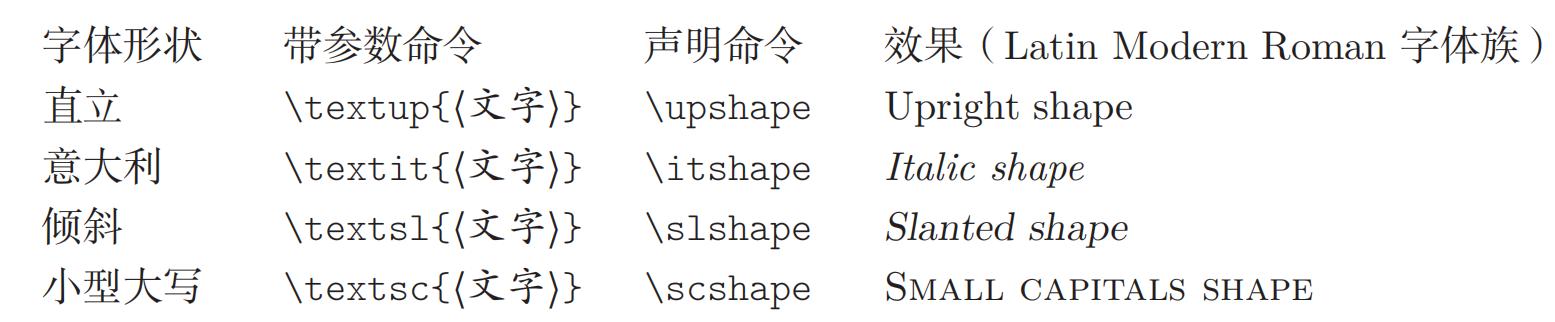
\includegraphics[width=0.8\textwidth]{字体形状.png}
\end{figure}

正文默认使用直立字体形状。注意其中倾斜形状和意大利形状的区别,倾斜形状差不多是直接对符号倾斜产生的,而通常所说的“斜体”往往指意大利形状,它类似于更加圆滑的手写体。因为数学公式的字体一般使用意大利形状,因而与数学混排时倾斜形状不会与公式的字母混淆;在标题、参考文献中也有使用倾斜形状的。并非所有字体族都有这么多形状,除了 \LaTeX 默认的 Computer Modern 和 Latin Modern ,大多数字体都只有意大利形状与倾斜形状的一种;很多字体也可能缺少小型大写字符的符号。另一方面,一些其他字体可能也会提供更多的字体形状,如 Venturis ADF 系列字体就提供倾斜的小型大写 ( italic small capitals )、空心( outline )等形状。

预定义命令的字体系列有中等 ( medium ) 和加宽加粗( bold extended )两类:
\begin{table}[H]
    \centering
    \begin{tabular}{ccccccc}
        字体系列 && 带参数命令 && 声明命令 && 效果 \\ 
        中等 && \verb|\textmd{文字}| && \verb|\mdseries| && \textmd{Medium series} \\ 
        加宽加粗 && \verb|\textbf{文字}|  && \verb|\bfseries| && \textbf{Bold extended series} \\
    \end{tabular}
\end{table}

正文默认使用中等字体系列。两个命令表示的意义对不同套字体可能有所区别,如命令 \verb|\textbf| 和
 \verb|\bfse| \verb|ries| 对默认的字体选择加宽加粗的字体系列,但对一些则是选择加粗( bold )或半粗( demi-bold )字体系列。

字体的这三种性质有如确定字体的三维坐标,同一维度的性质不能叠加,但不同类的性质则可以。三种性质的组合效果见下表:

\begin{figure}[H]
    \centering
    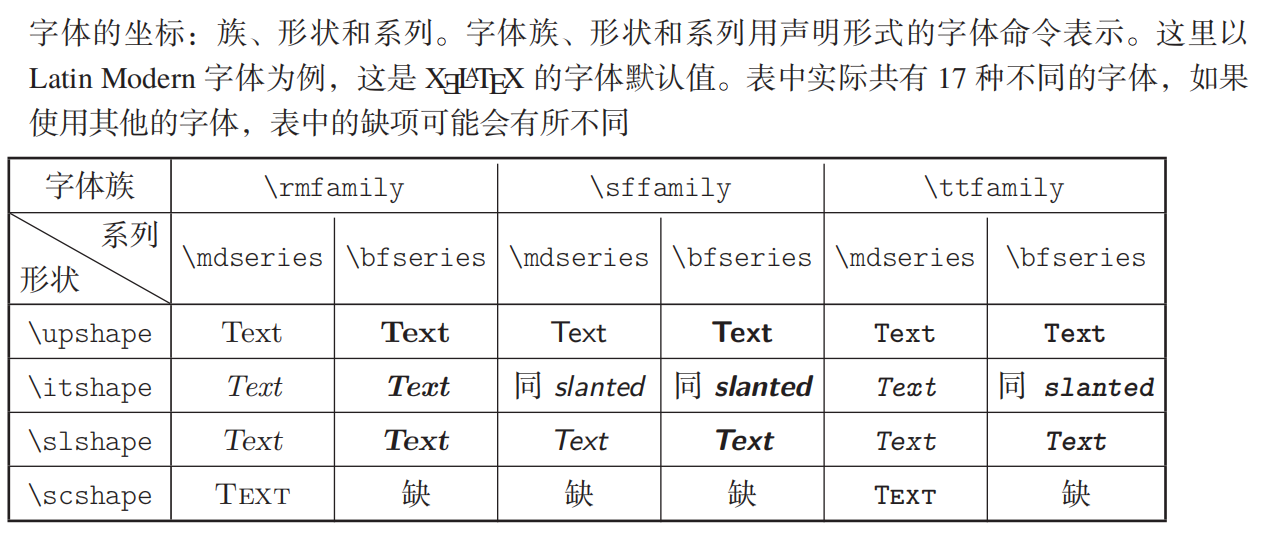
\includegraphics[width=0.85\textwidth]{字体三维坐标.png}
\end{figure}

除了上面列举的这些字体命令,还有\verb|\textnormal{文字}| 和 \verb|\normalfont| 命令用来把字体设置为“普通”的格式。默认情况下,普通字体相当于\verb|\rmfamily \mdseries \upshape| 的效果。普通字体特别适于在复杂的字体环境中恢复普通的字体,尤其是在宏定义这类不知道外部字体设置的情况下,如:

\begin{minipage}[t]{0.45\textwidth}
\begin{lstlisting}
\sffamily
\textbf{This is a pararaph of bold and \textit{italic font, sometimes returning to \textnormal{normal font} is necessary. }}
\end{lstlisting}
\end{minipage}
\hfill
\begin{minipage}[t]{0.45\textwidth}
    \sffamily
    \textbf{This is a pararaph of bold and \textit{italic font, sometimes returning to \textnormal{normal font} is necessary. }}
\end{minipage}

使用斜体声明 ( \verb|\itshape| 、\verb|\slshape| 时,最后一个倾斜的字母会超过右边界,使得后面的文字与它相距过紧,而用带参数的命令( \verb|\textit| 、 \verb|\textsl| 就可以自动修正这个距离,也可以手工使用 \verb|\/| 命令进行这种倾斜校正 ( italic correction ),如:

\begin{minipage}[t]{0.45\textwidth}
\begin{lstlisting}
{\itshape M} M

\textit{M}M

{\itshape M\/}M
\end{lstlisting}
\end{minipage}
\hfill
\begin{minipage}[t]{0.45\textwidth}
    {\itshape M}M

    \textit{M}M
    
    {\itshape M\/}M
\end{minipage}
倾斜校正命令\verb|\/| 会在字母后面加上一个小的距离,其大小由具体的字体和符号来决定。倾斜校正一般只用在声明形式的斜体命令中,但偶尔也使用它取消连字,也可以用来校正一些粗体字母和引号之间的距离(当然最好还是使用带命令的参数形式):

\begin{minipage}[t]{0.45\textwidth}
\begin{lstlisting}
Bold `{\bfseries leaf}'

Bold `{\bfseries leaf\/}'

Bold `\textbf{leaf}'
\end{lstlisting}
\end{minipage}
\hfill
\begin{minipage}[t]{0.45\textwidth}
Bold `{\bfseries leaf}'

Bold `{\bfseries leaf\/}'

Bold `\textbf{leaf}'
\end{minipage}

在很少的情况下,\verb|\textit| 自动加入的倾斜校正是不必要的,此时可以使用\verb|\nocorr| 命令禁止校正,如:

\begin{minipage}[t]{0.45\textwidth}
\begin{lstlisting}
\textit{M}M

\textit{M\nocorr}M
\end{lstlisting}
\end{minipage}
\hfill
\begin{minipage}[t]{0.45\textwidth}
    \textit{M}M

    \textit{M\nocorr}M
\end{minipage}

也可以使用 \verb|\renewcommand| 重定义\verb|\nocorrlist| 命令设置不对特定字符校正,\LaTeX 默认定义不对句号和逗号校正,相当于已经定义了:
\begin{lstlisting}
\newcommand{\nocorrlist}{,.}
\end{lstlisting}


中文字体通常没有西文字体那样复杂的成套的字体,各个字体之间一般都是独立的,只有少数字体有不同重量的成套字体。因此,对于中文字体,一般只使用不同的字体族进行区分。 xeCJK 和 CJK 宏包机制下,中文字体的选择命令和西文字体是分离的,选择中文字体族通常用 \verb|CJKfamily| 命令\footnote{还是不知道怎么用},如:

\begin{minipage}[t]{0.45\textwidth}
\begin{lstlisting}
{\CJKfamily{hei} 这是黑体}

{\CJKfamily{kai} 这是楷体}
\end{lstlisting}
\end{minipage}
\hfill
\begin{minipage}[t]{0.45\textwidth}
    {\heiti 这是黑体}

    {\kaishu 这是楷体}
\end{minipage}

中文的字体族,根据不同的系统和使用方式各有不同。在 \verb|ctex| 宏包及文档类下有一些预定义,在默认情况下( \verb|winfonts| 选项,针对 Windows 常用字体配置了的四种字体族:\verb|song|(宋体)、\verb|hei|(黑体)、\verb|kai|(楷书)、\verb|fs|(仿宋);如果使用了其他选项,则可能会有不同字体,为了方便实用,\verb|ctex| 宏包提供了简化的命令:

\begin{minipage}[t]{0.45\textwidth}
\begin{lstlisting}
{\songti 宋体} \quad {\heiti 黑体} \quad
{\fangsong 仿宋} \quad {\kaishu 楷书}
\end{lstlisting}
\end{minipage}
\hfill
\begin{minipage}[t]{0.45\textwidth}
    {\songti 宋体} \quad {\heiti 黑体} \quad
    {\fangsong 仿宋} \quad {\kaishu 楷书}
\end{minipage}

ctex 宏包及文档类(如 ctexart )另外定义了一些组合字体,可以让中文也具备使用粗体 (\verb|\bfseries|) 和意大利体 (\verb|\itshape| 的功能,并且重定义 \verb|rmfamily| 使它同时对中文起作用。默认的中文字体族是 \verb|rm| ,粗体是黑体,意大利体是楷体,如:

\begin{minipage}[t]{0.45\textwidth}
\begin{lstlisting}
% ctex 宏包下默认相当于 \CJKfamily{rm}
% \rmfamily 或 \textrm 也会同时设置此字体
中文字体的\textbf{粗体}与\textit{斜体}
\end{lstlisting}
\end{minipage}
\hfill
\begin{minipage}[t]{0.45\textwidth}
中文字体的\textbf{粗体}与\textit{斜体}
\end{minipage}

类似地,\verb|\sffamily| (对应 \verb|sf| 中文字体族)和\verb|ttfamily| (对应\verb|tt| 中文字体族)也可以同时作用于西文和中文,分别相当于幼圆和仿宋体。

\LaTeX 的这种利用相互正交的几种性质来区分字体的方式,称为新字体选择方案( New Font Selection Scheme ,NFSS)。当然,NFSS 最早于 1989 年发布,现在也并不新了;它是针对 Plain \TeX 和旧版本的\LaTeX 2.09 中直接制定具体字体旧方案而说的。在旧的字体选择方案中,一个字体命令对应一个单一的字体,甚至有些字体命令对应的字体的大小也是确定的,如在 Plain \TeX 和旧版本的\LaTeX 2.09格式中,命令\verb|\rm| ,\verb|\bf| ,\verb|\it| 分别表示使用 Computer Modern 的普通罗马字体、粗罗马字体和意大利体,但使用\verb|\bf\it| 并不能得到加粗的意大利体,而仍然只是一个\verb|\it| 的效果。NFSS 改变了这种不便的使用方式。现在,出于对旧文档的兼容考虑,现在的版本 \LaTeX 2$\epsilon$ 在标准文档类中也保留了 \verb|\rm| ,\verb|\bf| ,\verb|\it|,\verb|\sc|,\verb|\sl|,\verb|\sf|,\verb|\tt|等命令(以及数学模式底下的\verb|\mit|,\verb|\cal| 命令),请不要在文档中使用它们。

NFSS 为字体划分了编码,族,系列,形状,尺寸等多个正交属性,这些属性各自可以用一个简短的命令来表示。如字体编码有\verb|OT1,T1,OML,OMS,OMX,U|等;字体族有\verb|cmr,cmss,cmtt,cmm,cmsy,cmex|等;字体系列有 \verb|m,b,bx,sb,c|等;字体形状有\verb|n,it,sl,sc|等,由具体的字体可以有不同的定义,常用的标准定义可参见NFSS的标准文档、Adobe PostScript 字体文档。 \LaTeX 提供了更原始的命令:
\begin{lstlisting}
\fontencoding{编码}
\fontfamily{族}
\fontseries{系列}
\fontshape{形状}
\fontsize{大小}{基本行距} (纯数字,单位是 pt)
\end{lstlisting}

通过这些命令来使用这些属性,需要在后面加\verb|\selectfont| 命令使它们生效,如:

\begin{minipage}[t]{0.45\textwidth}
\begin{lstlisting}
\fontencoding{OT1} \fontfamily{pzc}
\fontseries{mb} \fontshape{it}
\fontsize{14}{17} \selectfont
PostScript New Century Schoolbook
\end{lstlisting}
\end{minipage}
\hfill
\begin{minipage}[t]{0.45\textwidth}
    \fontencoding{OT1} \fontfamily{pzc}
    \fontseries{mb} \fontshape{it}
    \fontsize{14}{17} \selectfont
    PostScript New Century Schoolbook
\end{minipage}

也可以使用
\begin{lstlisting}
    \usefont{编码}{族}{系列}{形状}
\end{lstlisting}
一次性选择某个字体,如:

\begin{minipage}[t]{0.45\textwidth}
\begin{lstlisting}
\usefont{T1}{pbk}{db}{n}
PostScript Bookman Demibold Normal
\end{lstlisting}
\end{minipage}
\hfill
\begin{minipage}[t]{0.45\textwidth}
    \usefont{T1}{pbk}{db}{n}
    PostScript Bookman Demibold Normal
\end{minipage}

\subsubsection{使用更多字体}

使用 \verb|\rmfamily,\bfseries,\itshape,\kaishu| 这类命令时,只能选择预定义的少数几种字体。对于西文,就是 Computer Modern 或 Latin Modern 系列的几款成套的字体;对于中文,就是 6 种预定义的 Windows 字体。这些对于简单的文章并没有问题,但如果想改变文章的整体风格,或者缺少预装的字体文件(如中文 Linux 用户就不会有 Windows 预装的中文字体),那么就需要用到预设之外的更多字体。

选择非默认的字体的方法有两类:当不使用 XeTeX 引擎时,可以通过字体宏包或 \LaTeX 底层字体命令调用在 \TeX 系统中安装的中西文字体;当使用 XeTeX 引擎时,可以调用操作系统安装的中西文字体。由于质量可靠的中文字体几乎都是商用的,因此 \TeX 系统中只安装了很少几种质量较差的中文字体,一般总要调用操作系统中的字体来使用 XeTeX 引擎的功能。

一个\TeX 发行版通常都同时安装了大量的西文字体,直接使用 \LaTeX 底层命令指定字体通常很难用,特别是一些字体同时还包括对应的数学字体和符号命令的设置,非常繁琐,因此很多西文字体都做成了方便调用的字体宏包,可以直接更换整套的西文字体(或数学字体)。其中,最为常见的要求是把整套字体换为 Times Roman 的衬线字体(罗马体)或  Helvetica 的无衬线字体,Times 字体也能与中文宋体很好地配合。有几个宏包可以达到这个目的,最简单的是 times 宏包,只更换正文字体,没有更换配套的数学字体,很少使用; mathptmx 在 times 宏包的基础上增加了数学字体的支持;效果最好的免费字体则是 txfonts 宏包,对整套西文字体和数学符号给出了完整的解决方案。使用字体宏包非常简单,通常只需要导入该宏包即可:

\begin{lstlisting}
\documentclass{article}
\usepackage{txfonts}
\begin{document}
Test text
\end{document}
\end{lstlisting}

txfonts 的效果见图 \ref{fig:txfonts}。

\begin{figure}[H]
    \centering
    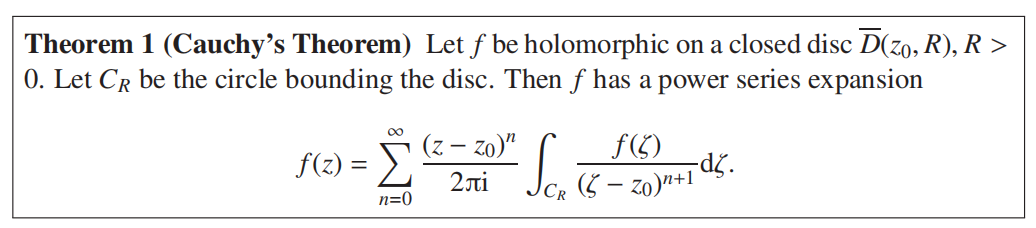
\includegraphics[width=0.9\textwidth]{字体1.png}
    \caption{Times 字体效果( txfonts )}
    \label{fig:txfonts}
\end{figure}

为文章的不同部分选用字体应该协调配合,因此通常带有配套数学字体的字体包时最为常用的,但有时也需要分别定义正文字体和与之配套的数学字体,此时就必须手工指定不同的字体包,例如使用高德纳的 Concrete 正文字体与 Zapf 的 Euler 数学字体配合时(这正是 Concrete 字体设计时的用法),就需要综合使用字体包 ccfonts 和 euler:

\begin{lstlisting}
\usepackage{article}
\usepackage{T1}{fontenc}
\usepackage{ccfonts,eulervm}
\begin{document}
Test text
\end{document}
\end{lstlisting}

这一字体组合比较清晰,它与无衬线字体包(如 arev , cmbright )都比较适合于在幻灯片演示中使用,效果见图\ref{fig:euler}

\begin{figure}[H]
    \centering
    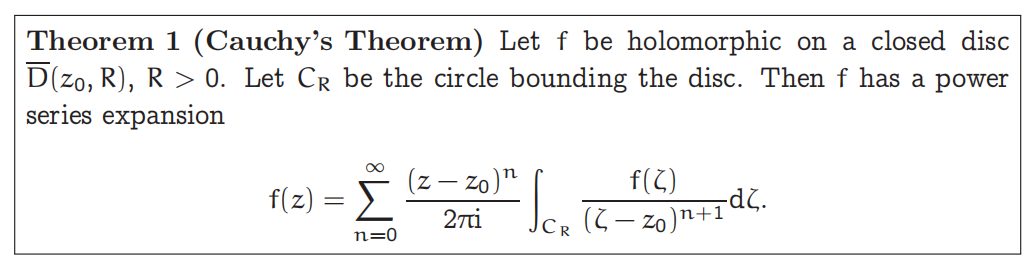
\includegraphics[width=0.9\textwidth]{字体2.png}
    \caption{Concrete 字体和 Euler 字体效果( T1 编码,ccfonts,euler)}
    \label{fig:ruler}
\end{figure}

在使用 Concrete 与 Euler 字体时,我们使用了一个新的宏包 fontenc 来选择字体的编码。 fontenc 宏包可以包含多个选项,表示文档所使用的正文字体编码,最后一个选项的编码是文档默认使用的编码。字体的编码决定字体包含的符号,同一组的字体可能有不同编码的版本。除了 XeLaTeX 使用的 Unicode 编码(在 NFSS 中一般是 EU1 ),传统的 \LaTeX 字体编码有一般正文字体 OT1 、 拓展正文字体 T1 、 数学字母 OML 、 数学符号 OMS 、数学符号拓展 OMX 等。需要手工设置的通常只有正文字体的编码,默认的正文字体编码是 OT1 , 而拓展编码 T1 则包含更多的符号,特别是带重音的拉丁字母等。许多字体包都要求使用 T1 编码,才能获得更好的效果,在字体包的说明文档中一般都会提及。注意字体编码是指符号在字体中位置的编码,与输入文档使用的文档编码不是一回事。

初拥 \LaTeX 的最大的问题往往是并不知道 \LaTeX 中哪些字体可用,因为作为一门排版语言,\LaTeX 并没有把可用的字体放在一个下拉菜单中等待选择,因此必须自己查看 \TeX 发行版的字体安装目录或综述性的字体文档。一个带有说明、例子、使用方法和详细功能比较的综述性文档是 Stephen 的 HartkeFree\_Math\_Font\_Survey\footnote{\href{https://www.ctan.org/tex-archive/info/Free\_Math\_Font\_Survey/en}{https://www.ctan.org/tex-archive/info/Free\_Math\_Font\_Survey/en}},里面介绍了 20 多种带有数学支持的免费 \TeX 字体。该文档在 \texlive 和 CTeX 套装中都有收录 , 是使用成套字体的很好的参考。一个收录更为全面的 \LaTeX 字体目录是 FontCatalogue \footnote{\href{https://tug.org/FontCatalogue/}{https://tug.org/FontCatalogue/}},它展示了 Linux 源中的 \texlive 所能使用的近 200 种西文字体族。

下面来看现代的方法,使用 XeTeX 来选择字体。在 XeLaTeX 中,主要使用 fontspec 宏包的机制来调用字体。最基本的是设置正文罗马字体族、无衬线字体族和打字机字体族的命令:

\begin{lstlisting}
    \setmainfont[可选选项]{字体名}
    \setsansfont[可选选项]{字体名}
    \setmonofont[可选选项]{字体名}
\end{lstlisting}

(可用的可选选项参见 fontspec 文档 \footnote{\href{https://ctan.org/tex-archive/macros/unicodetex/latex/fontspec}{https://ctan.org/tex-archive/macros/unicodetex/latex/fontspec}} )

例如:
\begin{lstlisting}
    % 在导言区设置全文学体为 Windows 提供的
    % Times New Roman, Verdana, Courier New 字体
    \usepackage{fontspec}
    \setmainfont{Times New Roman}
    \setsansfont{Verdana}
    \setmonofont{Courier New}
\end{lstlisting}

此时\verb|\rmfamily| ,\verb|\sffamily|和\verb|\ttfamily| 就分别对应设置的三种字体,而且 fontspec会自动找到并匹配对应的粗体、斜体等变体,尽量使 \verb|\bfseries|,\verb|\itshape|等命令也有效。

也可以定义新的字体族命令:
\begin{lstlisting}
    \newfontfamily{命令}[可选选项]{字体名}
\end{lstlisting}

例如为Java运行库附带的 Lucida Sans 字体定义一个命令\verb|\lucidasans| :

\begin{minipage}[t]{0.45\textwidth}
\begin{lstlisting}
% 导言区使用
\newfontfamily{\lucidasans}{Lucida Sans}
% 正文使用
{\lucidasans This is Lucida Sans.}
\end{lstlisting}
\end{minipage}
\hfill
\begin{minipage}[t]{0.45\textwidth}
\begin{figure}[H]
    \centering
    
\includegraphics[width=0.8\textwidth]{lucida.png}
\end{figure}
\end{minipage}

XeLaTeX 下中文字体的设置使用 xeCJK 宏包(ctex宏包或文档类会自动调用它)。xeCJK 提供了与 fontspec 对应的中文字体设置命令:
\begin{lstlisting}
    \setCJKmainfont[可选选项]{字体名}
    \setCJKsansfont[可选选项]{字体名}
    \setCJKmonofont[可选选项]{字体名}
    \setCJKfamilyfont{中文字体族}[可选选项]{字体名}
\end{lstlisting}

这些命令对于 Linux 等系统下的中文用户特别有用,因为 ctex 宏包默认是针对 Windows的字体配置的,可以用 \verb|nofonts| 选项禁用预定义的中文字体设置而来自已定义字体,例如使用文鼎公司免费发布的字体:
\begin{lstlisting}
    % 在导言区设置全文字体为 “文鼎 PL 报宋 GBK”
    % 并设置中文的 kai 字体族为 “文鼎 PL 简中楷”
    \setCJKmainfont{AR PLBaosong2GBK Light}
    \setCJKfamilyfont{kai}{AR PL KaitiM GB}
\end{lstlisting}

此后使用 \verb|\CJKfamily{kai}|就会使用文鼎的楷体。

fontspec 所能使用的字体是 fontconfig 库所能找到的所有字体,也就是在 \TeX 发行版和操作系统中所安装的字体,通常是 OpenType 和 TrueType 的字体,也包括一些 PostScript 格式字体,需要注意的就是要使用正确的字体名。字体的列表可以在命令行下使用 fc-1st 命今来列出,通常列出的学体信息会非多,不能在一屏内完全显示。 Windows 下还会因编码不统一品出现乱码,此时可以利用命令重定向操作符把结果输
出到文件中:
\begin{lstlisting}
    fc-list > fontlist.txt
\end{lstlisting}

\verb|fc-list|命令输出的结果类似这样(这里只选取了一小部分,并稍做重新排列):

\begin{lstlisting}
D:/application/texlive/2023/texmf-dist/fonts/truetype/public/dejavu/DejaVuSerifCondensed-Italic.ttf: DejaVu Serif,DejaVu Serif Condensed:style=Condensed Italic,Italic
D:/application/texlive/2023/texmf-dist/fonts/opentype/public/domitian/Domitian-Bold.otf: Domitian:style=Bold
D:/application/texlive/2023/texmf-dist/fonts/opentype/google/roboto/RobotoSerif-ExtraLight.otf: Roboto Serif,Roboto Serif ExtraLight:style=ExtraLight,Regular
D:/application/texlive/2023/texmf-dist/fonts/opentype/public/drm/drmdozittc9.otf: drmdozittc9:style=Regular
D:/application/texlive/2023/texmf-dist/fonts/opentype/public/drm/drmdozl7.otf: drmdozl7:style=Regular
D:/application/texlive/2023/texmf-dist/fonts/opentype/public/cm-unicode/cmunoti.otf: CMU Concrete:style=Italic
D:/application/texlive/2023/texmf-dist/fonts/opentype/public/archivo/Archiv0-MediumItalic.otf: Archiv0 Medium:style=Medium Italic,Italic
D:/application/texlive/2023/texmf-dist/fonts/opentype/public/kerkis/Kerkis-BoldSmallCaps.otf: Kerkis:style=BoldSmallCaps
C:/Windows/fonts/LHANDW.TTF: Lucida Handwriting:style=Italic,kursiv,Cursiva,Kursivoitu,Italique,Corsivo,Cursief,Itálico
C:/Windows/fonts/vgasysr.fon: System:style=Regular
\end{lstlisting}

\verb|fc-1ist|列出的是字体名(对应于字体族)和同族字体变体(对应于 \LaTeX 的字体系列和形状)。在冒号前面的是字体族名称,\verb|style=|后面的是字体的变体,用逗号分隔开的是同一个字体(或变体)在不同语言下的名称。通常 fontspec 宏包会自动处理好字体的变体,因此只要知道前面的字体名称。

\verb|fc-1ist|可以带许多参数来控制输出的格式。例如,我们通常只需要字体族名而不需要变体的名称,就可以加\verb|-f"%{family}\n"|选项只输出字体族;又如,使用\verb|:lang=zh|选项可以只输出中文学体,而\verb|:outline|则可以只显示矢量字体。下面的命
令就可以将所有中文字体族的列表输出到 \verb|zhfont.txt|中:
\begin{lstlisting}[language=sh]
    fc-list -f "%{family}\n" :lang=zh > zhfont.txt
\end{lstlisting}

fontspec 宏包为字体,尤其是 OpenType 字体提供了多种字体性质的选项。例如 Minion Pro 字体使用带斜线的数字 0,以与字母 O 区分:

\begin{minipage}[t]{0.45\textwidth}
\begin{lstlisting}
\newfontfamily{\minion}[Numbers=SlashedZero]{Minion Pro}
\minion 100, 0K
\end{lstlisting}
\end{minipage}
\hfill
\begin{minipage}[t]{0.45\textwidth}
\begin{figure}[H]
    \centering
    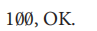
\includegraphics[width=0.3\textwidth]{minion.png}
\end{figure}
\end{minipage}

字体选项的选择可参见 The XeTeX Companion-TeX meets OpenType and Unicode \footnote{ \href{https://xml.web.cern.ch/XML/lgc2/}{https://xml.web.cern.ch/XML/lgc2/}} 、fontspec 宏包文档 \footnote{\href{https://ctan.org/pkg/fontspec}{https://ctan.org/pkg/fontspec}}。OpenType
字体提供的性质可通过命令行工具 \verb|otfinfo|或 opentype-info 宏包查看。

对中文字体来说,尤其有用的一组 fontspec 命令选项是设置斜体、粗体、粗斜体的选项\verb|ItalicFont|,\\
\verb|BoldFont|,\verb|BoldItalicFont|,这几个选项可以把字体的变体用另一种字体来代替。如可以设置正文学体为宋体,其粗体为黑体、斜体为楷体,粗斜体为隶书,以弥补中文字体一般没有一族成套变体的问题:

\begin{lstlisting}
\setCJKmainfont[BoldFont=SmHei,ItalicFont=KaiTi,BoldItalicFont=LiSu]{SimSun}
\end{lstlisting}

ctex 宏包默认设置 Windows 字体时正是采用类似以的方法。如果不指定中文字体的变体形式,ctex 调用 xeCJK 时会增加选项使用伪粗体和伪斜体代替。不过中文排版没有斜体的概念,因此在非 Windows环境一般也都需要设置这种中文的复合字体,避免斜体的使用。

fontspec 主要用于设置正文字体,通常不用来设置数学字体,不过一些数学字体(如\verb|\mathrm|)默认与正文字体一致,则正文字体的设置会影响到数学字体。 fontspec 的\verb|\setmathrm|,\verb|\setmathsf|,\verb|\setmathtt|等命令可以用来以与正文同样的方式设置这些受影响的数学字体,它们的用法和\verb|\setmainfont|等命令类似。此外, fontspec 宏包的 \verb|no-math| 选项可以禁用其对数学字体的所有影响(包括\verb|\setmahtrm|等命令的作用),在加载许多数学字体包时,这个选项都会自动生效,对于不自动加载\verb|no-math|选项的宏包,我们可以自已加上这个选项。为了使用正确的字体编码,fontspec 应该放在数学字体包的后面。当然,fontspec 几乎总会令字体宏包原来的正文字体设置失效,可以使用 fontspec 的方式再另行设置搭配的字体,例如:
\begin{lstlisting}
    \documentclass{article}
    \usepackage{ccfonts} %公式使用 Concrete 系列字体
    \usepackage[no-math]{fontspec} % \mathrm 等也使用 Concrete 系列字体
    \setmainfont{Latin Modern Mono Prop} % 正文使用 Latin Modern Mono 字体
\end{lstlisting}

处理中文时的情况可能更复杂一些。如果使用 xeCJK 或 ctex/ctexcap 宏包,可以在它们之前使用数学字体包,需要时可以带 \verb|no-math| 选项加载fontspec,用法和前面西文的文档类似。使用 ctex 中文文档类时,如果需要,fontspec 的no-math选项可以传递给文档类。当 fontspec 是由文档类加载时,就不可能在这之前加载数学字体包了,但由于个别字体包会改变字体编码,此时可能需要在数学字体包之后以 EU1 编码为最后一个选项加载 fontenc 宏包,以保证使用正确的字体编码,例如:
\begin{lstlisting}
\documentclass[no-math]{ctexart}
\usepackage[utopia]{mathdesign} % 数学字体使用 mathdesign 与 Utopia
\usepackage[EU1]{fontenc} % 恢复正文字体的 Unicode 编码
\setmainfont{Utopia Std} % 正文字体使用 OpenType 格式的 Adobe Utopia
\end{lstlisting}

在使用数学字体包时同时加载对应的 OpenType 或 TrueType 格式的正文字体,是在 XeLaTeX 下使用复杂字体的一般方法。

一种更方便的方式是使用传统的字体包设置全文的字体(数学或正文字体),只把其他字体(如汉字)留给 fontspec 和 xecJK 。也就是说,我们要将旧的字体选择机制和新的学体选择机制混合使用,这同样可以做到,与前面的区别仅仅是使用 fontenc 宏包将传统的 Unicode字体编码设置为默认的编码,即最后一个选项。这种方法不影响使用 fontspec 中\verb|\newfontfamily|声明的字体和 XeTeX 声明的汉字字体。但 \verb|\setmainfont|,\verb|setsansfont| 和 \verb|setmonofont| 这三人命令会因字体编码而失效,需要时在文档中使用\verb|\fontencoding|命令临时切换编码,或者直接重定义\verb|\rmfamily|、\verb|\sffamily|和\verb|\ttfamily|,让它们增加切换编码的功能。下面给出一个在设置字体方面比较复杂的例子,以西文的 T1 编码为默认编码调 fourier 字体包,西文用 fontspec 的两种方式定义其他字体,汉字也使用 OpenType 的字体:
\begin{lstlisting}
    \documentclass[UTF8]{ctexart}
    % 西文正文和数学字体
    \let\hbar\relax % 解决 xunicode 与 fourier 的符号冲突
    \usepackage{fourier}
    % 设置默认编码为 T1,以支持fourier 宏包
    \usepackage[T1]{fontenc}
    % 定义新的西文 Times 字体族
    \newfontfamily{\times}{Times New Roman}
    % 设置西文等宽字体,并重定义 \ttfamily 来切换到 EU1 编码
    \setmonofont{Consolas}
    \let\oldttfamily\ttfamily
    \def\ttfamily{\oldttfamily \fontencoding{EU1} \selectfont}
    % 设置中文字体
    \setCJKmainfont{Adobe Kaiti Std}
    \begin{document}
    Utopia text and $\sum math$ fonts.
    汉字楷书与 {\times Times New Roman} 字体。
    \texttt{Consolas 0123}
    \end{document}
\end{lstlisting}

XeTeX 通常不影响符号字体包的使用,但偶尔会因为字体编码不同而造成问题:注意 XeTeX 在同一时刻只能使用一种字体编码,多种字体编码要手工切换。例如
通常由 fontspec 自动加载的 xunicode 宏包\footnote{现在好像不会自动加载了}会把国际音标字体包 tipa 的功能对应到 Unicode 编码字体上,但这会使原来的\verb|\textipa|命令改用 fontspec 管理的 Unicode 编码字体。因此默认的正文体 Latin Modern 因为符号不全就不能用于国际音标输出,应该改用包含音标符号的字体,如Linux Libertine O、Times New Roman等。例如:

\begin{lstlisting}
    % XeLaTeX 编译
    \documentclass[UTF8]{ctexart}
    % \usepackage{xunicode} 我这里加这行才能编译
    % 不需要 tipa 宏包,xunicode 已经实现其功能
    \setmainfont{CMU Serif} % Computer Modern Roman 的 Unicode 版本
    \begin{document}
    \LaTeX{}读音为\textipa{["lA:tEx]}。
    \end{document}
\end{lstlisting}

如果不愿意使用 OpenType 或 TrueType 格式的 Unicode 编码国际音标字体,仍然可以在 XeTeX 下使用 T3 编码的 tipa 的功能:

\begin{lstlisting}
    % XeLaTeX 编译
    \documentclass[UTF8]{ctexart}
    \usepackage{tipa} % 宏包已经正确加载fontenc
    % \mytipa 的定义参考原来的 \textipa 的旧定义,手工切换编码
    \newcommand\mytipa[1]{{\fontencoding{T3}\selectfont#1}}
    \begin{document}
    \LaTeX{}读音为\mytipa{["lA:tEx]}。
    \end{document}
\end{lstlisting}

有时调用一个字体并没有对应的字体包,就必须通过文档了解字体在 NFSS 下的坐标,手工进行选定。如使用 Computer Modern 的 Fibonacci 字体,就可以直接设置字体族:

\begin{minipage}[t]{0.45\textwidth}
\begin{lstlisting}
    \fontfamily{cmfib} \selectfont
    Computer Modern Fibonacci Roman
\end{lstlisting}
\end{minipage}
\hfill
\begin{minipage}[t]{0.45\textwidth}
    \fontfamily{cmfib} \selectfont
    Computer Modern Fibonacci Roman
\end{minipage}

而如果要将 Fibonacci 字体设置为全文的默认字体,并且让\verb|\rmfamily|和\verb|\textrm|都指
向 Fibonacci 字体,就需要在导言区重定义默认的罗马字体族\verb|\rmdefault|:

\begin{lstlisting}
    % 导言区修改全文默认字体 Computer Modern Fibonacci 字体族
    \renewcommand\rmdefault{cmfib}
\end{lstlisting}

类似地,可以重定义\verb|\sfdefault|和\verb|\ttdefault|来修改\verb|\rmfamily|和\verb|\ttfamily| 表示的字体族。进一步,如果希望让全文的默认学体是无衬线的字体族,那么还可以重定义\verb|\familydefault|,如:
\begin{lstlisting}
    % 导言区修改全文默认字体为无衬线字体族 phv(Helvetica)
    \renewcommand\familydefault{\sfdefault}
    \renewcommand\sfdefault{phv}
\end{lstlisting}

这正是 helvet 宏包的主要工作。当然,在有对应宏包的情况下,还是应该尽量使用宏包提供的功能,这样可能有针对特定字体的更详细的设置。

类似地,较新版本的 XeTeX 也提供 \verb|\CJKrmdefault|,\verb|\cJKsfdefault|,\verb|\CJKttdefault| 和\\ \verb|\CJKfamilydefault| 命令,其用法与 NFSS 中的几个命令类似。在排版中文文档时,如果重定义了\\\verb|\familydefault|设置全文为无衬线字体族,那么也应该同时设置中文:
\begin{lstlisting}
    \renewcommand\CJKfamilydefault{\CJKsfdefault}
\end{lstlisting}

最后介绍一个有用的宏包 fonttable,可以用它输出字体的符号表,这对于使用\verb|\symbol|命令时查找符号代码特别有用。在导言区使用
\begin{lstlisting}
    \usepackage{fonttable}
\end{lstlisting}
之后, 就可以使用命令
\begin{lstlisting}
    \fonttable{原始字体名}
    \xfonttable{编码}{族}{系列}{形状}
\end{lstlisting}
得到字体的符号表。例如,我们可以列举出 T1 编码下 Latin Modern Roman 的字体符号表:
\begin{lstlisting}
    \xfonttable{T1}{lmr}{m}{n}
\end{lstlisting}

\xfonttable{T1}{lmr}{m}{n}

